\documentclass[11pt,a4paper,openany]{report}
\usepackage[T1]{fontenc}
\usepackage[utf8]{inputenc}
\usepackage{lmodern}
\usepackage{microtype}
\usepackage{amsmath,amssymb,amsthm,mathtools,bm}
\usepackage{booktabs,array,longtable,tabularx}
\usepackage{xcolor}
\usepackage[margin=22mm,headheight=23pt]{geometry}
\usepackage{enumitem}
\usepackage{fancyhdr}
\usepackage{graphicx}
\usepackage{url,xurl,hyperref}
\definecolor{finblue}{HTML}{1F5A99}
\definecolor{fingreen}{HTML}{19733A}
\definecolor{finorange}{HTML}{D55E00}
\definecolor{finred}{HTML}{A61B1B}
\definecolor{finviolet}{HTML}{6A3D9A}
\definecolor{fingray}{HTML}{4D4D4D}
\hypersetup{
  unicode=true,colorlinks=true,linkcolor=finblue,citecolor=fingreen,urlcolor=finblue,
  pdftitle={FIN Research Programs P394--P410},
  pdfauthor={Krzysztof Żuchowski},
  pdfsubject={Formal boundary, contact geometry, noisy operational design, and an executable Jordan-sampling specification},
  pdfkeywords={FIN, Lean, Sturm theorem, Lindemann-Weierstrass, photonic identifiability, quantum discrimination, Jordan sampling, operational physics}
}
\pagestyle{fancy}
\fancyhf{}
\fancyhead[L]{\small FIN Programs P394--P410}
\fancyhead[R]{\small Release 10.34}
\fancyfoot[C]{\thepage}
\setlength{\parindent}{0pt}
\setlength{\parskip}{0.55em}
\setlist{nosep,leftmargin=2em}
\setcounter{tocdepth}{2}
\setcounter{secnumdepth}{3}
\emergencystretch=3em
\newcommand{\R}{\mathbb R}
\newcommand{\N}{\mathbb N}
\newcommand{\statusProven}{\textcolor{fingreen}{[Proven]}}
\newcommand{\statusStrong}{\textcolor{finblue}{[Strong evidence]}}
\newcommand{\statusConditional}{\textcolor{finviolet}{[Conditional]}}
\newcommand{\statusRefuted}{\textcolor{finred}{[Refuted]}}
\newcommand{\statusBlocked}{\textcolor{finorange}{[Blocked by external evidence]}}

\begin{document}
\hypersetup{pageanchor=false}
\begin{titlepage}
\centering
\vspace*{8mm}
{\Large\bfseries FIN --- Release 10.34\par}
\vspace{9mm}
{\Huge\bfseries Research Programs P394--P410\par}
\vspace{6mm}
{\Large Formal boundary, contact geometry, noisy operational design,\par
and an executable Jordan-sampling specification\par}
\vspace{14mm}
{\Large Krzysztof \.{Z}uchowski\par}
\vspace{2mm}
{\normalsize Independent Researcher --- Fractal Information Theory Project\par}
\vspace{2mm}
{\normalsize ORCID: \href{https://orcid.org/0009-0002-0909-3613}{0009-0002-0909-3613}\par}
\vspace{7mm}
{\large 31 July 2026\par}
{\normalsize Publication --- Preprint; Version 1.0.0\par}
\vfill
\begin{minipage}{0.93\textwidth}
\small
\textbf{Exact contact geometry.} The frozen degree-eleven dual has nine
critical points in $(0,1)$, isolated by exact rational Sturm arithmetic.
Every one of the seven P366 primal atoms has strictly positive complementary
slack; the displayed primal/dual pair is near-contact, not exact-contact.

\textbf{Operational completion.} A frozen JSON protocol, event schema,
validator, hashes, and 50,000 synthetic events implement the Jordan Sampling
Realization. The software passes; physical evidence is explicitly not
admitted.

\textbf{Boundary.} No selector, full legacy-to-strict bridge, dimensional
source, role transfer, calibrated laboratory realization, Standard Model,
gravity, or Theory-of-Everything closure is claimed.

\medskip
\textbf{Repository.} \url{https://github.com/hyconiek/Fractal-Nadsoliton-Theory}

\textbf{License.} CC BY 4.0.
\end{minipage}
\vfill
\end{titlepage}
\hypersetup{pageanchor=true}
\pagenumbering{roman}

\chapter*{Publication statement}
\addcontentsline{toc}{chapter}{Publication statement}
This monograph reports every executed Program P394--P410 and recommends
Programs P411--P427. Mathematical proof, proof-kernel reflection, numerical
evidence, conditional operational construction, and external empirical
admission are kept distinct. The legacy/strict split and current strict-core
guardrails remain binding.

\tableofcontents
\clearpage
\pagenumbering{arabic}

\chapter*{Abstract}
\addcontentsline{toc}{chapter}{Abstract}

This monograph executes FIN Research Programs P394--P410 without reopening
exhausted selector, generic bridge, role-transfer, dimensional-source, or
total-action loops.

P394 reflects the complete depth-fourteen Bernstein subdivision algorithm
through Lean. Exact de Casteljau arithmetic visits 147 adaptive nodes and
certifies the full tree whose unpruned frontier contains 16,384 cells.
Taylor, fifth-root generation, and the P366 Krawczyk map remain outside the
end-to-end formalization.

P395 proves by exact rational Sturm arithmetic that the degree-ten derivative
of the P380 dual has exactly nine roots in $(0,1)$, each isolated in a box of
width at most $2^{-50}$. Six are near active constraints and three are
inactive. Exact interval evaluation at all seven P366 primal atom boxes gives
strictly positive complementary slack. The smallest lower slack is
$5.54\times10^{-10}$. Thus the frozen P366/P380 pair is near-contact but not
an exact complementary pair. P395 then solves a new simultaneous
25-equation contact system. Its residual is $3.42\times10^{-28}$ and its
objective is $0.7073534677231137$, but its Jacobian condition number is
$2.73\times10^{15}$; interval certification remains open.

P396 isolates the strict-kernel injectivity proof as a reduction to
Lindemann--Weierstrass linear independence of four exponentials. P397 then
refutes exactly one proposed source class for the damping completion atom:
it is not a multiplicative character of additive distance.

P398 searches for distant compensating aliases from four starts in a wide
66-loss/66-phase chart. Every fit returns near the canonical origin and no
distant alias candidate is found; the best transfer defect is
$4.32\times10^{-6}$. This is a nonexhaustive atlas, not a global theorem.

P400 optimizes permutation-symmetric pure codebooks under dephasing and
improves the better product/GHZ baseline by up to $0.06138$. P401 performs a
full twelve-mode one-use search and finds no improvement over the extremal
two-mode input in the supplied isotropic noise. P402 solves twelve finite-grid
clock maximin designs; the best worst-case feasible distance is $0.99999047$.

P403 provides both a custody-aware executable experiment contract and a
separate 50,000-event moment-reconstruction integration test. Both pass while
physical evidence remains false. P404 proves the JSR-specific law
$I(S;X)=H_2(q_-)$, equal to $0.874517$ bits here. P405 constructs a
conditional sign-phase encoder but refutes its interpretation as an
increasing negativity monotone or non-premise selector. P406 proves a unique
outer scale only after the quarter-tail normalization $1/4$ is supplied.

P399 and P407--P410 remain external evidence gates. The strongest surviving
interpretation is a rigorous finite spectral and signed-moment framework with
an executable operational interface, whose conversion into physics still
requires physical references, standards, apparatus, and independent data.

\chapter*{Confidence convention}
\addcontentsline{toc}{chapter}{Confidence convention}
\begin{center}
\small
\begin{longtable}{@{}p{0.26\textwidth}p{0.64\textwidth}@{}}
\toprule
\textbf{Label} & \textbf{Meaning}\\
\midrule
\endhead
\statusProven & Mathematical proof, exact arithmetic, kernel-checked terminal predicate, or exhaustive finite result.\\
\statusStrong & Reproducible bounded or high-precision computation with explicit limitations.\\
\statusConditional & Requires a named encoding, apparatus law, calibration, clock, standard, or axiom.\\
\statusRefuted & The declared proposition fails in its stated class.\\
\statusBlocked & Independent data, hardware, custody, standards, or unblinding is required.\\
\bottomrule
\end{longtable}
\end{center}

\chapter{Scope and guardrails}

\section{Kernel split}

The legacy intermediate kernel is
\[
K_{\mathrm{legacy,ont}}(d)
=4\ln2\frac{\cos(\pi d/4+\pi/6)}{1+0.01d},
\]
whereas the strict working kernel is
\[
K_{\mathrm{strict,gate}}(d)
=\frac{\cos((743/4000)d+13/80)}{1+d^{9/5}}.
\]
They are not silently identified. P397 audits only one source class for the
already target-defined attenuation completion atom. It neither derives the
strict kernel from the legacy kernel nor transfers any legacy physical role.

\section{Ontology and observer boundary}

The internal order remains
\[
\text{nadsoliton}\longrightarrow\text{light}\longrightarrow\text{matter}
\longrightarrow\text{emergent observer}.
\]
The nadsoliton is primordial information in a solitonic state, with no lower
informational substrate. A common self-adjoint generator can generate both
$e^{-itA}$ and $e^{-tA}$, but functional calculus does not itself specify a
physical state, clock, apparatus, environment, instrument, or record.

\section{Open boundaries preserved}

This report does not claim:
\begin{itemize}
\item QW-2191 discharge or a non-premise selector;
\item a source-independent complete legacy-to-strict map;
\item transfer of legacy electroweak, electromagnetic, or hierarchy roles;
\item internal length, time, action, mass, or energy standards;
\item a calibrated twelve-state laboratory realization or vertex POVM;
\item a unit-bearing nonproxy $L_{\mathrm{total}}$;
\item Standard Model, gravity, or Theory-of-Everything closure.
\end{itemize}

\chapter{Executive results}

\small
\begin{longtable}{@{}p{0.09\textwidth}p{0.58\textwidth}p{0.22\textwidth}@{}}
\toprule
\textbf{Program} & \textbf{Principal result} & \textbf{Status}\\
\midrule
\endhead
P394 & Complete Bernstein subdivision algorithm reflected by Lean & Proven; remaining generators open\\
P395 & Exact old-dual audit plus 25-equation KKT candidate & Proven audit; strong candidate\\
P396 & Four-exponential injectivity reduction & Proven externally; local LW formalization open\\
P397 & Additive-character damping source excluded & Proven in one class\\
P398 & Four-start wide-box alias atlas; no distant candidate & Moderate evidence\\
P399 & Independent photonic pilot absent & Blocked\\
P400 & Symmetric codebook improves product/GHZ baselines & Strong evidence\\
P401 & Full twelve-mode search finds no one-use multimode gain & Strong evidence\\
P402 & Twelve clock-error maximin designs & Proven finite-grid result\\
P403 & Custody contract plus moment validator & Proven computation; physical execution blocked\\
P404 & JSR negativity-to-information law & Proven within JSR\\
P405 & Sign-phase identity; not selector or negativity monotone & Proven; refuted interpretation\\
P406 & Unique scale after supplied quarter-tail law & Conditional; canonicity refuted\\
P407--P410 & QW, standards, reservoir, and EW records absent & Blocked\\
\bottomrule
\end{longtable}
\normalsize

\chapter{P394: algorithm-reflected Bernstein feasibility}

P394 moves the complete depth-fourteen Bernstein subdivision algorithm into
Lean. Each cell stores twelve exact integer numerators and a positive common
denominator. De Casteljau splitting at one half and the denominator update
are recomputed exactly. A node is pruned only when all its Bernstein
coefficients lie in $[-1,0]$.

The full unpruned frontier contains 16,384 cells. Adaptive execution visits
147 nodes and the Lean kernel proves that the recursive certificate returns
true. This is algorithm reflection, not merely terminal predicate checking.

A companion source checks twenty-two exact terminal fifth-root brackets, but
their generation remains Python-side. The trust boundary is:
\begin{center}
\small
\begin{longtable}{@{}p{0.50\textwidth}p{0.37\textwidth}@{}}
\toprule
\textbf{Layer} & \textbf{Status}\\
\midrule
\endhead
Complete Bernstein recursive algorithm & Lean-kernel checked\\
Terminal fifth-root inequalities & Lean-kernel checked\\
Generation of fifth-root endpoints & Python implementation\\
Moment cosine Taylor/Lagrange bounds & Python implementation\\
P366 Krawczyk map and interval propagation & Python implementation\\
Lindemann--Weierstrass theorem & External theorem\\
\bottomrule
\end{longtable}
\end{center}
P394 fully reflects one algorithm while explicitly leaving the other
generators open.

\chapter{P395: exact contact topology}

Let $p(x)=\sum_{j=0}^{11}a_jx^j$ be the frozen rational P380 dual polynomial,
already certified to lie in $[-1,0]$ on $[0,1]$. The rational Sturm chain of
$p'$ proves
\[
\#\{x\in(0,1):p'(x)=0\}=9.
\]
Every root lies in a rational box of width at most
$2^{-50}=8.88\times10^{-16}$.

\begin{center}
\small
\begin{longtable}{@{}r r r r@{}}
\toprule
\textbf{No.} & \textbf{$x$ midpoint} & \textbf{$p(x)$ midpoint} & \textbf{Boundary distance}\\
\midrule
\endhead
1 & 0.0198303330 & -0.9999999793 & $2.07\times10^{-8}$\\
2 & 0.1294250512 & $-5.08\times10^{-9}$ & $5.08\times10^{-9}$\\
3 & 0.2003754633 & -0.0588238886 & 0.0588\\
4 & 0.2950459798 & $-3.22\times10^{-10}$ & $3.22\times10^{-10}$\\
5 & 0.4144591497 & -0.0835768539 & 0.0836\\
6 & 0.5266937250 & $-1.80\times10^{-9}$ & $1.80\times10^{-9}$\\
7 & 0.6905262847 & -0.3540308952 & 0.3540\\
8 & 0.8140624992 & $-7.54\times10^{-9}$ & $7.54\times10^{-9}$\\
9 & 0.9418431582 & -0.9999999395 & $6.05\times10^{-8}$\\
\bottomrule
\end{longtable}
\end{center}

Six points are near active boundaries and three are inactive. Exact rational
interval evaluation on the five Krawczyk node boxes and two fixed nodes gives
strictly positive complementary slack at every primal atom. The smallest
certified lower slack is
\[
5.53659989375616\times10^{-10}.
\]
The frozen primal and dual therefore cannot be an exact complementary pair,
although their objective gap remains below $3.05\times10^{-8}$.

P395 then moves all six interior nodes, seven weights, and twelve dual
coefficients simultaneously. The 25-equation KKT candidate has contact
pattern
\[
(-1,0,0,0,0,-1,0),
\]
objective $0.7073534677231137$, and maximum 80-digit residual
$3.42\times10^{-28}$. Its smallest double-precision Jacobian singular value
is $4.99\times10^{-13}$ and its condition number is
$2.73\times10^{15}$. Severe ill-conditioning prevents theorem status:
interval Krawczyk inclusion and global Bernstein feasibility remain required.

\begin{figure}[ht]
\centering
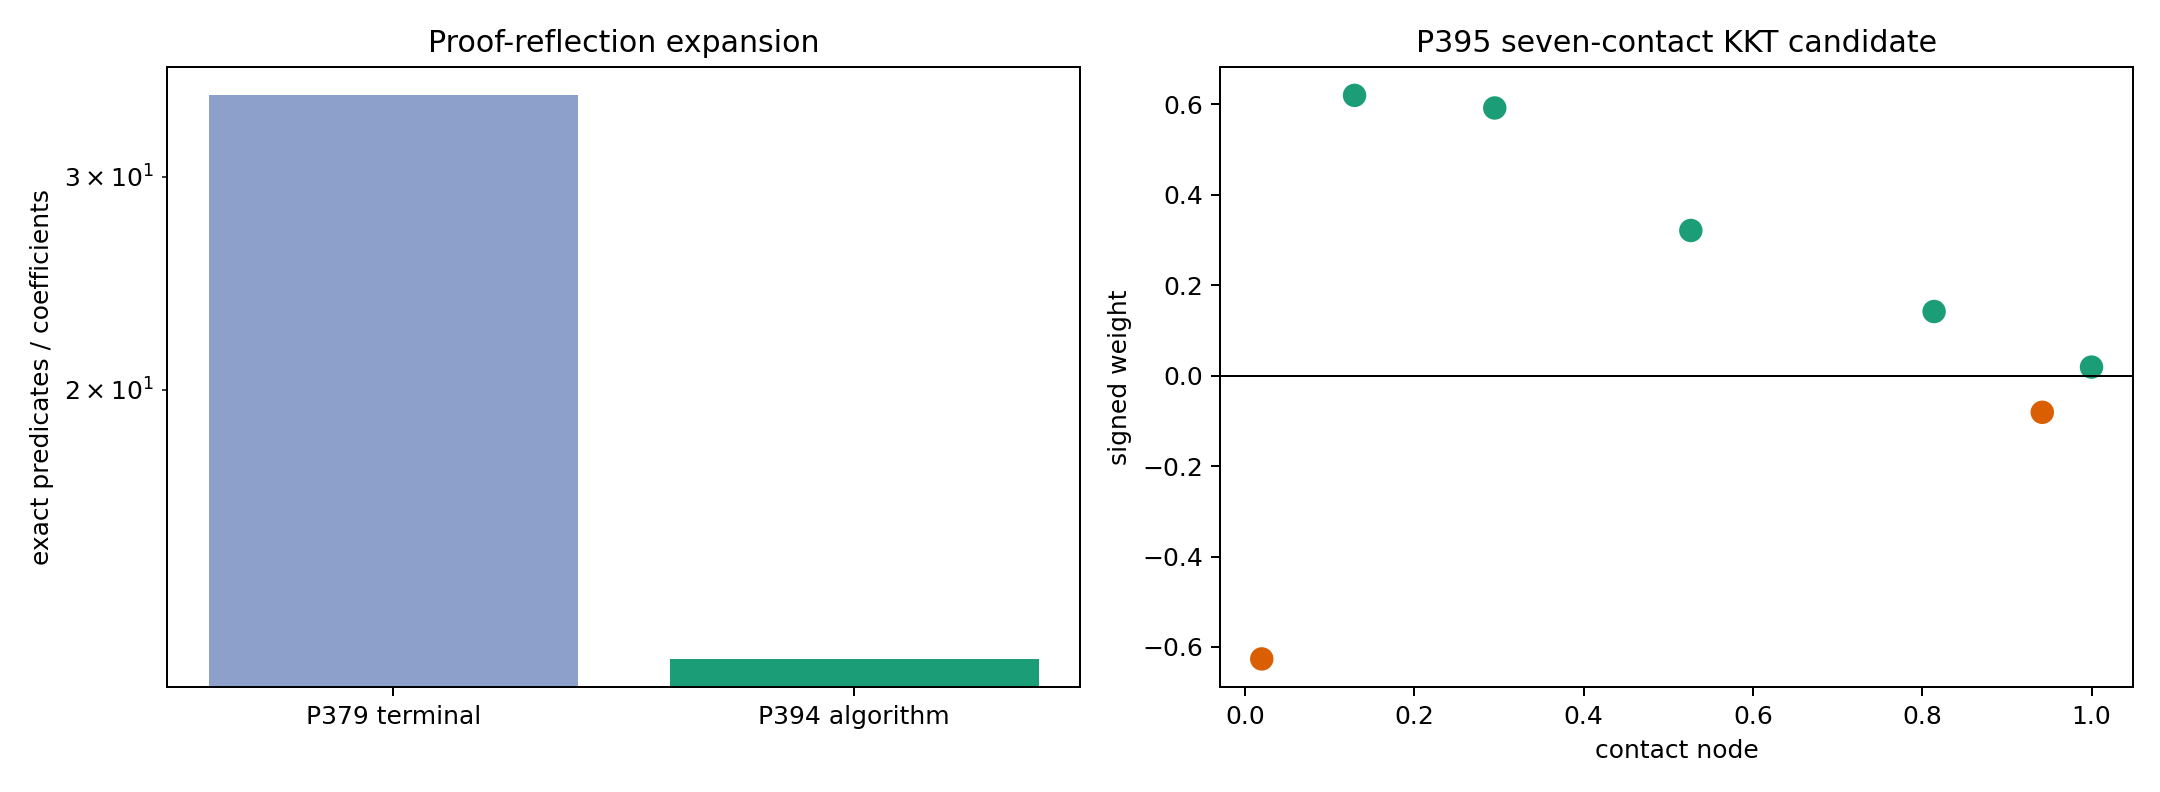
\includegraphics[width=0.97\textwidth]{FIN_Programs_394_410_Figures/p394_p395_reflection_contact.png}
\caption{P394 algorithm reflection and the P395 seven-contact KKT candidate.}
\end{figure}

\chapter{P396: injectivity and its formal boundary}

For integer $d\ge0$, define
\[
x_d=\frac{743d+650}{4000},\qquad
a_d=\frac{1}{1+d^{9/5}}.
\]
If $K_{\mathrm{strict}}(d)=K_{\mathrm{strict}}(e)$, then
\[
a_de^{ix_d}+a_de^{-ix_d}-a_ee^{ix_e}-a_ee^{-ix_e}=0.
\]
For $d\ne e$, the four exponents $ix_d,-ix_d,ix_e,-ix_e$ are distinct
algebraic numbers, and the coefficients are nonzero algebraic numbers.
Lindemann--Weierstrass linear independence forbids the relation. Hence the
strict kernel is injective on $\N_0$.

The local Lean artifact checks the final structural implication once the
independence premise is supplied. It does not locally mechanize
transcendence theory. Full reflection requires a formal library for
algebraicity, distinctness, and Lindemann--Weierstrass.

\chapter{P397: one damping-source class fails}

The target-defined damping completion is
\[
C(d)=\frac{1+d/100}{1+d^{9/5}}.
\]
If it were a multiplicative character of additive distance, it would satisfy
$C(2)=C(1)^2$. Since
\[
C(1)=\frac{101}{200},\qquad
C(2)=\frac{51/50}{1+2^{9/5}},
\]
equality would force
\[
2^{9/5}=\frac{30599}{10201}.
\]
Taking fifth powers yields the exact contradiction
\[
30599^5-512\,10201^5
=-29731872867024874359513\ne0.
\]
Thus the entire positive additive-character source class is excluded by one
exact witness. This is not a no-go for nonlinear RG cocycles, nonlocal memory,
or another new typed source.

\chapter{P398--P399: photonic quotient and hardware boundary}

After quotienting exact $2\pi$ phase periodicity, P398 starts four searches in
the small chart
\[
\ell_j\in[0,0.03],\qquad \varphi_j\in[-0.1,0.1].
\]
The optimizer may move in
\[
\ell_j\in[0,0.5],\qquad \varphi_j\in[-\pi,\pi].
\]
All fits return to parameter norm of order $10^{-6}$. No distant alias meets
the $10^{-8}$ transfer gate; the best raw transfer defect is
$4.32\times10^{-6}$. Because the nonconvex optimizer does not reach the exact
canonical zero to machine precision, the correct reading is a bounded atlas
with no alias found, not global injectivity.

P399 remains blocked because no independent pilot with
raw timestamps, complex transfer tomography, calibration hash, custody, and
authorized unblinding is present.

\chapter{P400: noise-adapted symmetric codebooks}

For $n$ uses, a permutation-symmetric pure input is parameterized by Hamming
sector probabilities $p_0,\ldots,p_n$:
\[
|\psi_p\rangle=
\sum_{k=0}^{n}\sqrt{\frac{p_k}{\binom nk}}
\sum_{|x|=k}|x\rangle .
\]
Independent eigenbasis dephasing multiplies a matrix element by
$q^{d_H(x,y)}$. Across 64 settings with $n\le4$, the optimized symmetric
codebook improves the better product/GHZ baseline by as much as
\[
0.0613792.
\]
The maximum remaining gap to the hybrid adaptive upper bound is
\[
0.4926401.
\]
This is a nonconvex, ancilla-free, parallel, loss-free lower bound, not an
unrestricted adaptive optimum.

\begin{figure}[ht]
\centering
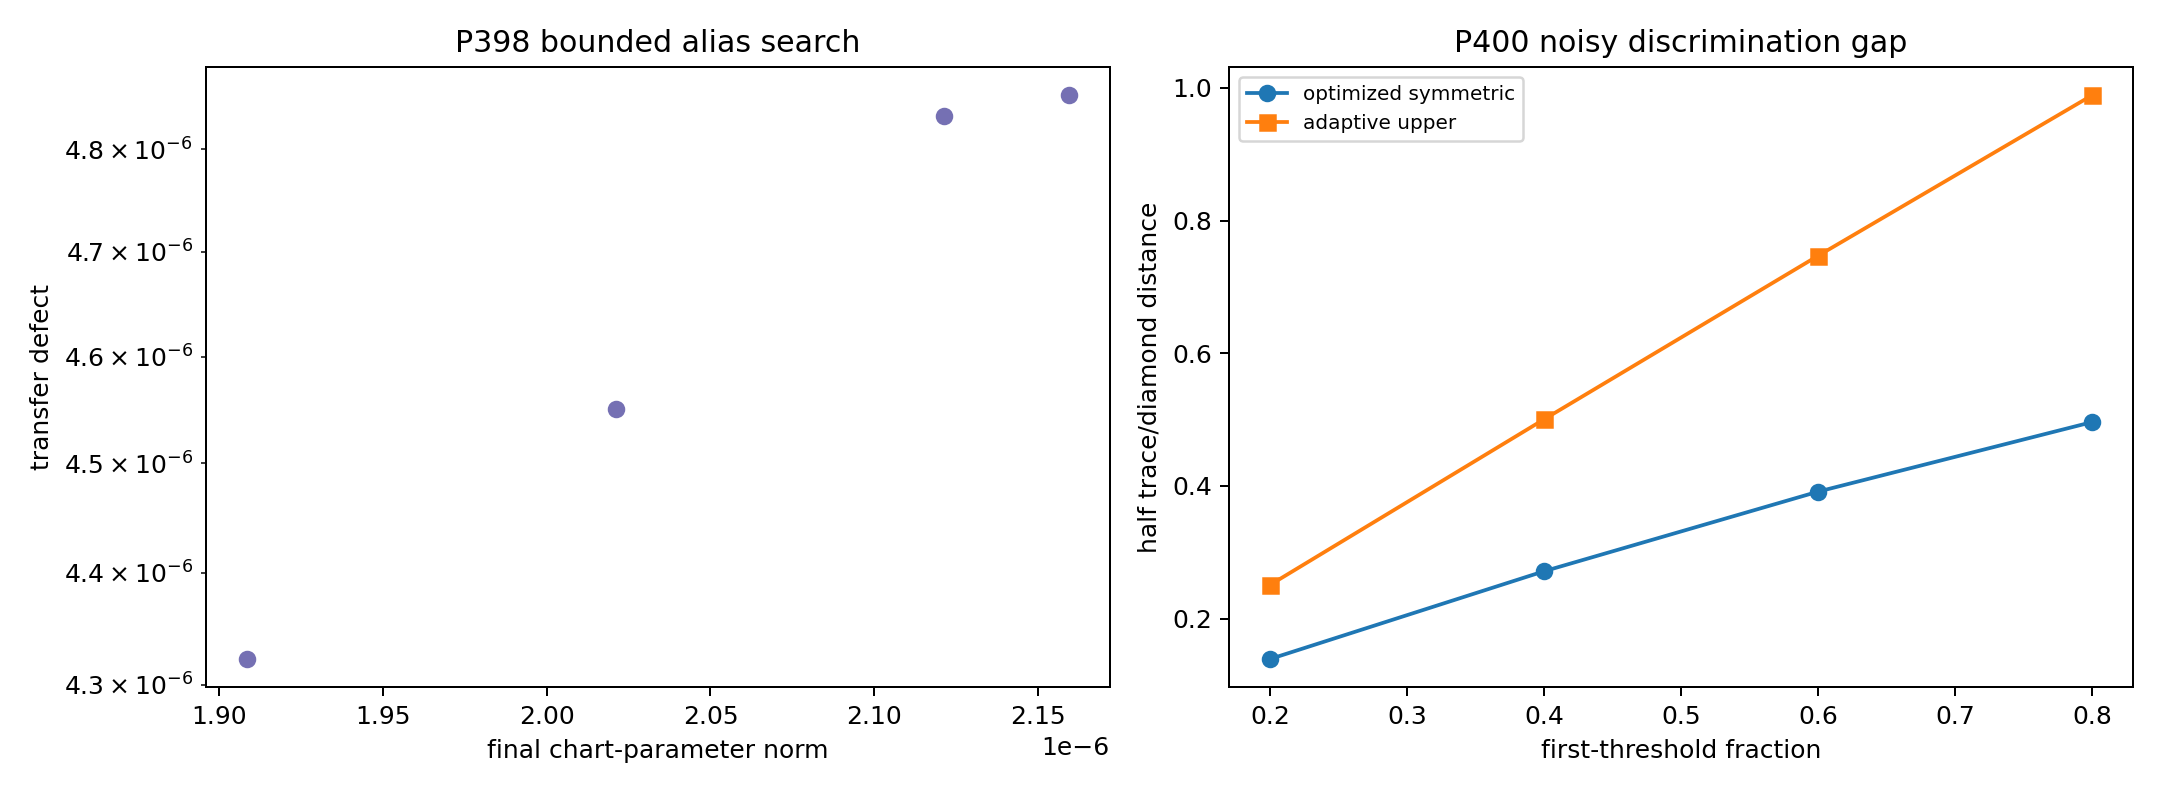
\includegraphics[width=0.97\textwidth]{FIN_Programs_394_410_Figures/p398_p400_alias_noise.png}
\caption{P398 bounded alias search and P400 symmetric-codebook gap.}
\end{figure}

\chapter{P401--P402: twelve modes and clock maximin design}

\section{Full twelve-mode one-use search}

The strict and amplitude-absorbed legacy circulant generators share a Fourier
basis. The relative generator is Fourier diagonal to defect
$5.07\times10^{-15}$. P401 optimizes an arbitrary probability vector over all
twelve modes for uniform off-diagonal dephasing $q$ and heralded survival
$\eta$.

Across 36 settings, no input improves on the equal superposition of the two
extremal relative-generator modes beyond reported numerical precision. This
negative result supports, but does not prove, one-use extremal-two-mode
optimality. Multiple adaptive uses and apparatus calibration remain open.

\section{Clock-error maximin schedules}

For every $n=1,\ldots,4$ and $q\in\{0.5,0.75,1\}$, P402 searches 1,501
nominal times on the first branch. With
$\delta\tau\in[-0.001,0.001]$, the objective is the smaller feasible
discrimination at the two endpoints. Twelve designs are solved; the best
worst-case value is $0.9999904711$.

This is exact only for the finite grid and supplied tube/noise model. It does
not create a physical time unit.

\begin{figure}[ht]
\centering
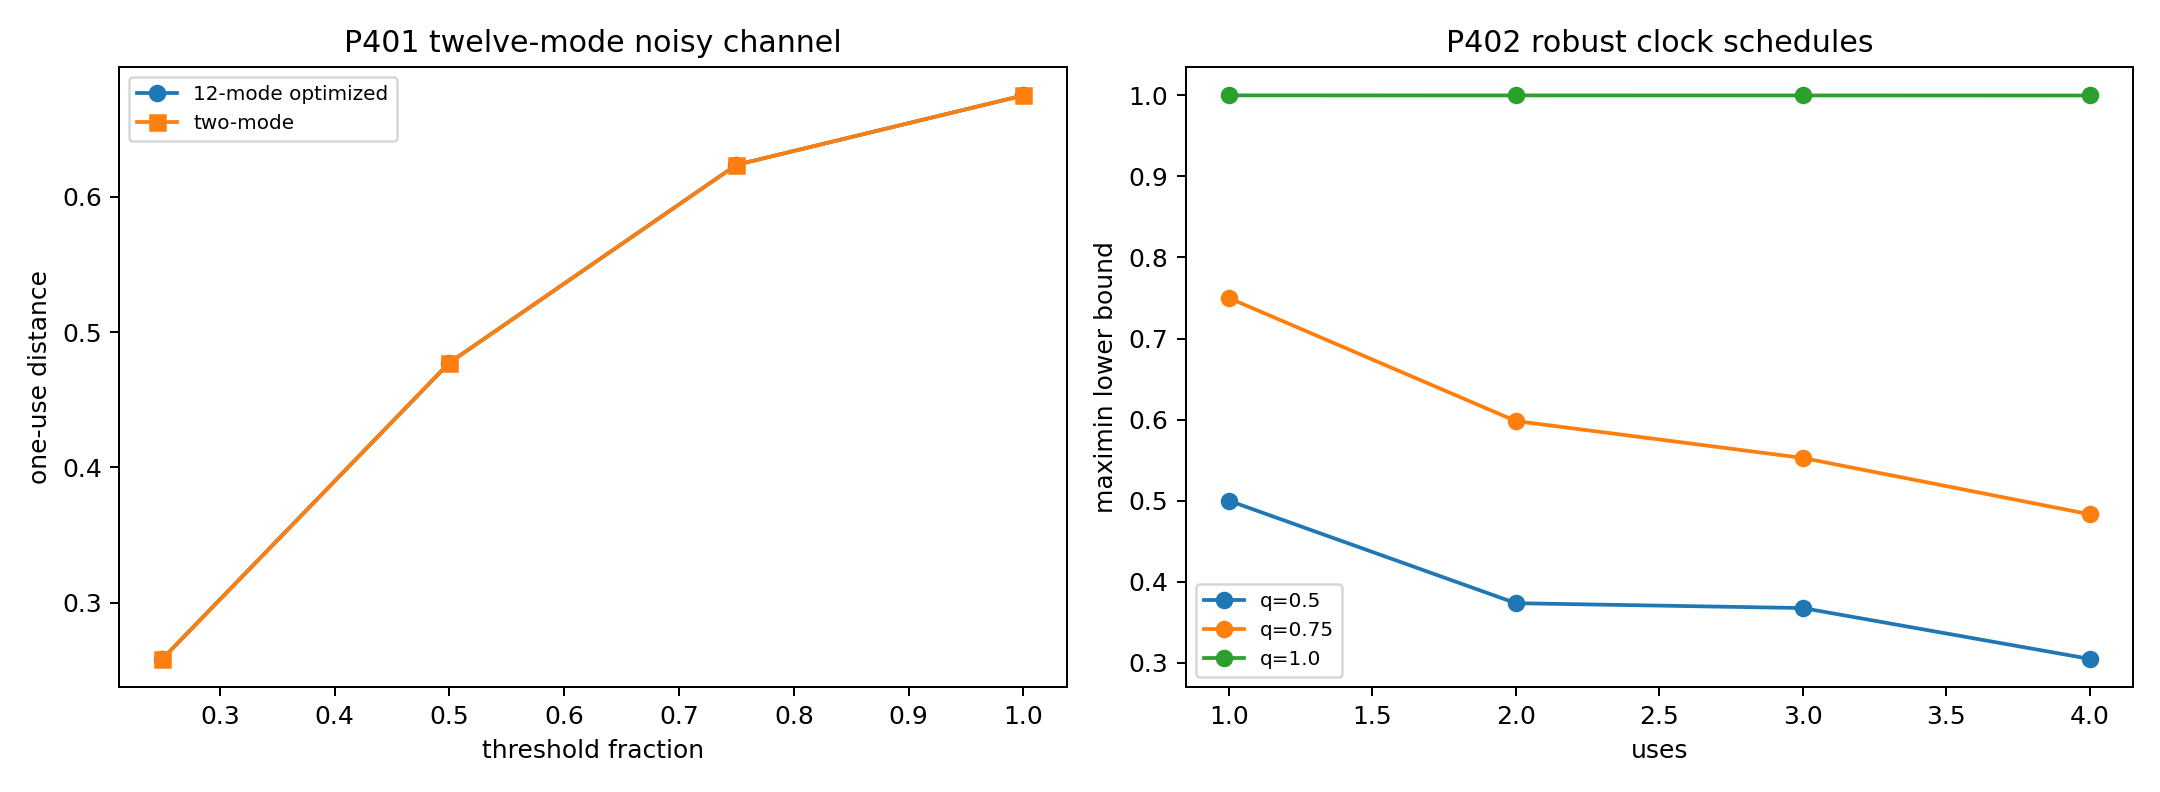
\includegraphics[width=0.97\textwidth]{FIN_Programs_394_410_Figures/p401_p402_full_mode_clock.png}
\caption{P401 twelve-mode search and P402 clock maximin schedules.}
\end{figure}

\chapter{P403: executable Jordan Sampling Realization}

For a finite signed measure $\mu=\sum_iw_i\delta_{x_i}$, let
\[
V=\sum_i|w_i|,\qquad q_i=\frac{|w_i|}{V},\qquad
s_i=\operatorname{sgn}(w_i).
\]
The event score for moment order $k$ is $Y_k=Vs_ix_i^k$, and
\[
\mathbb E_qY_k=\sum_iw_ix_i^k.
\]
All preparation probabilities are ordinary and nonnegative. The sign is a
classical importance-sampling register, not negative probability.

P403 freezes two complementary executable layers. The custody-aware transfer
contract consists of:
\begin{itemize}
\item \texttt{FIN\_P403\_JSR\_Executable\_Spec.json};
\item \texttt{fin\_p403\_jsr\_validator.py}.
\end{itemize}
It requires nine event fields, eleven manifest fields, three distinct roles,
hash-before-unblinding, one analysis run, and no model repair after failure.

The moment-reconstruction integration test consists of:
\begin{itemize}
\item \texttt{FIN\_P403\_Jordan\_Sampling\_Protocol.json};
\item \texttt{FIN\_P403\_Jordan\_Sampling\_Synthetic\_Events.csv};
\item \texttt{fin\_p403\_moment\_validator.py};
\item \texttt{FIN\_P403\_Jordan\_Sampling\_Validation.json}.
\end{itemize}
Each event contains event id, run id, timestamp tick, atom, node, and sign.
The validator checks schema, unique identifiers, strict timestamp order,
frozen atom identity, normalized probabilities, raw-record hash, empirical
atom frequencies, and twelve moment estimates.

For 50,000 synthetic events, the maximum moment $z$-score is 1.583. The
validation passes. The field
\texttt{physical\_evidence\_admitted} is false.

\begin{figure}[ht]
\centering
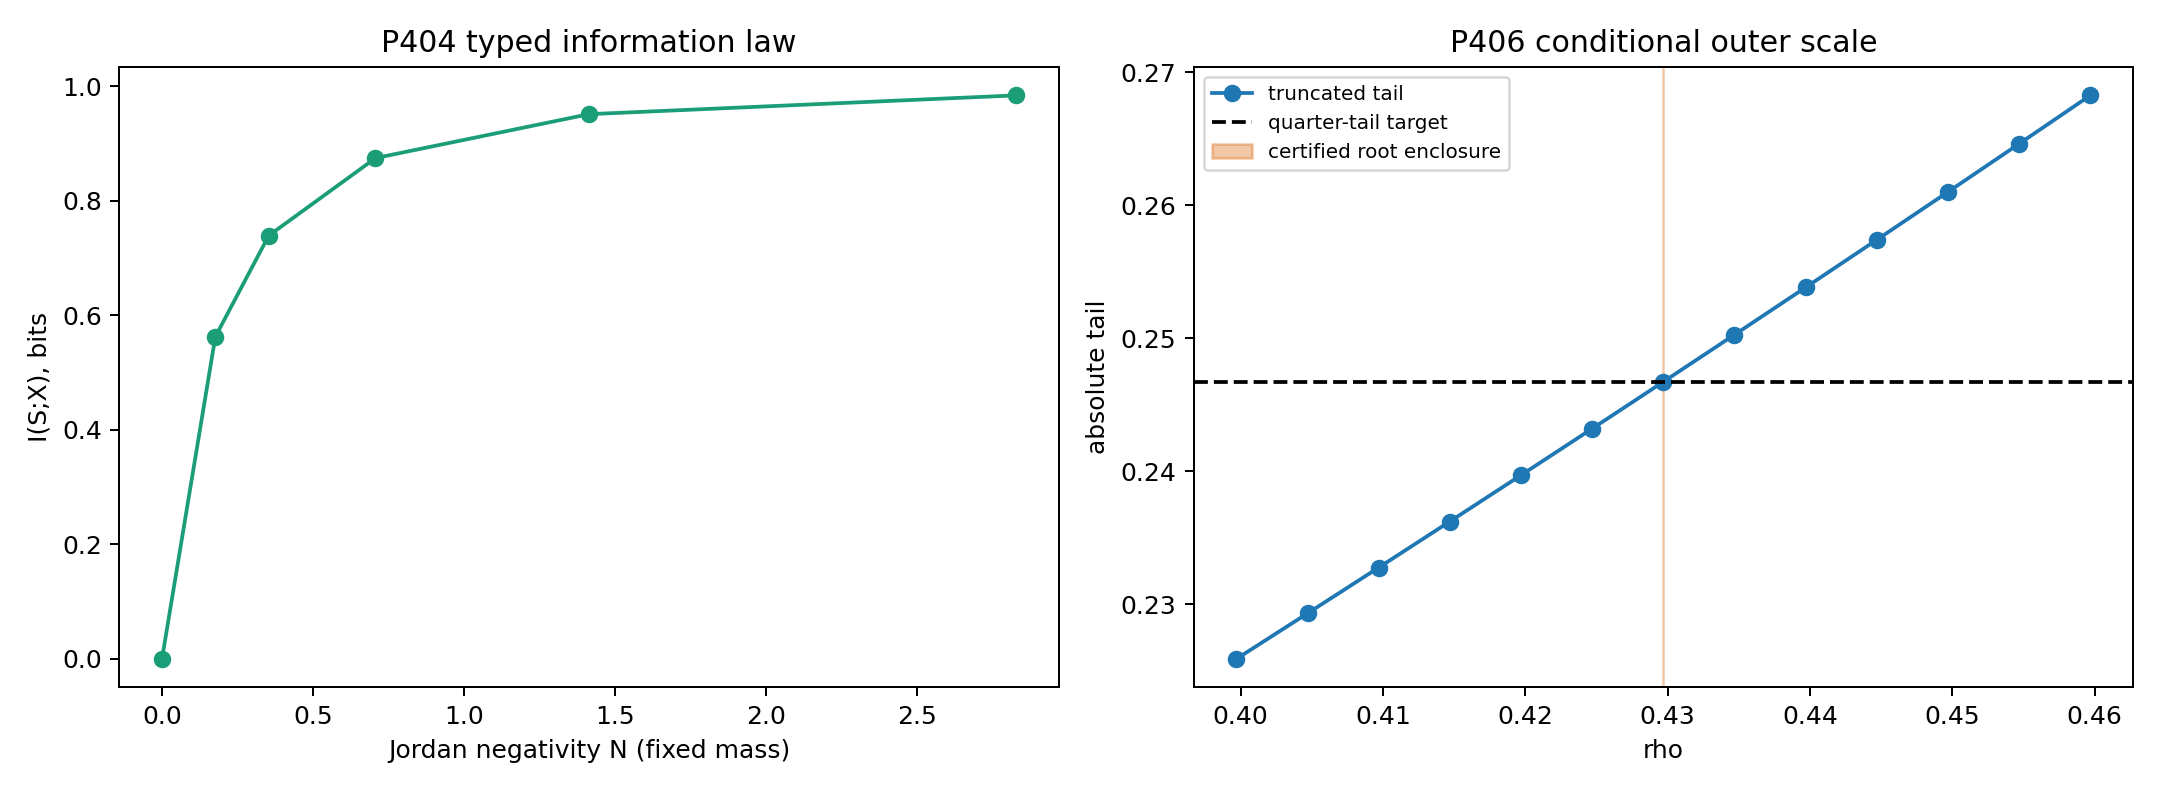
\includegraphics[width=0.97\textwidth]{FIN_Programs_394_410_Figures/p403_p406_jsr_information_scale.png}
\caption{P404 JSR information law and the P406 conditional outer section.}
\end{figure}

The synthetic bundle is an integration test, not laboratory evidence. The
structural self-test checks logic, not the truth of custody metadata. A real
execution must add independent preparation, apparatus, detector calibration,
custody, hold-out, and unmodified failure reporting.

\chapter{P404--P405: JSR information and conditional phase}

\section{Negativity-to-information law inside JSR}

For signed mass $m>0$ and Jordan negative mass $N\ge0$,
\[
q_- = \frac{N}{m+2N}.
\]
Because the atom determines its sign,
\[
I(S;X)=H_2(q_-).
\]
At fixed $m$, this increases with $N$ until $q_-=1/2$, and data processing
gives $I(S;Y)\le I(S;X)$. For the seven-atom object:
\[
m=0.9868259032,\quad N=0.7073534684,\quad
q_-=0.2945424925,\quad I(S;X)=0.8745170155\ {\rm bits}.
\]
This is specific to the JSR encoding and does not turn Shannon information
into thermodynamic entropy.

\section{Conditional sign-phase encoding}

Encode $s=+1$ as $|+\rangle$ and $s=-1$ as $|-\rangle$. The mixture obeys
\[
C_{l_1}(\rho_{\rm phase})
=\operatorname{TV}(p_S,\mathsf R p_S)
=|1-2q_-|.
\]
The value is 0.4109150151 for the certified object. At fixed positive mass it
decreases as negativity increases, so it is sign bias rather than an
increasing negativity monotone. Swapping the encoded basis reverses polarity
without changing magnitude. The basis/orientation is supplied and QW-2191
remains open.

\chapter{P406: quarter-tail normalized outer section}

Define
\[
F(\rho)=\sum_{d\ge1}|K_{\rm strict}(d)|\rho^d.
\]
P406 adds exactly one boundary law:
\[
F(\rho)=\frac{|K_{\rm strict}(0)|}{4}.
\]
The positive series is continuous and strictly increasing. A 160-term
truncation and
\[
0\le R_{160}(\rho)\le
\frac{\rho^{161}}{161^{9/5}(1-\rho)}
\]
give the unique conditional solution
\[
\rho\approx0.4296970877901551
\]
with computed enclosure width $2.30\times10^{-63}$. The factor $1/4$ is an
added, dimensionless normalization. It is not source-derived and creates no
length, action, mass, energy, or SI unit.

\chapter{External gates P407--P410}

No artifact satisfies the required provider, registrar, calibration-hash,
raw-record-hash, freeze-time, analyst, and unblinding fields for:
\begin{itemize}
\item P407: independent QW hold-out;
\item P408: dimensional standards;
\item P409: reservoir process tomography;
\item P410: electroweak blind test.
\end{itemize}
These are deliberately unfilled empirical slots. They require independent
people, apparatus, standards, and records.

\chapter{New theoretical objects}

\small
\begin{longtable}{@{}p{0.10\textwidth}p{0.31\textwidth}p{0.46\textwidth}@{}}
\toprule
\textbf{Object} & \textbf{Name} & \textbf{Exact boundary}\\
\midrule
\endhead
O131 & Algorithm-Reflected Bernstein Certificate & Other generators remain open\\
O132 & Seven-Contact KKT Extremal & Interval/global certification open\\
O133 & Transcendence Dependency Interface & Reduction, not local transcendence library\\
O134 & Additive-Character Damping Obstruction & One source class only\\
O135 & Bounded Photonic Alias Atlas & Four searches, not global/hardware\\
O136 & Noise-Adapted Symmetric Codebook & Restricted lower bound, not optimum\\
O137 & Twelve-Mode Noisy Discrimination Simplex & One use only; no lab\\
O138 & Noisy Clock Maximin Schedule & Frozen finite design only\\
O139 & JSR Executable Experiment Contract & Software/custody schema, not lab evidence\\
O140 & JSR Sign-Information Transformation & JSR-specific, not thermodynamics\\
O141 & Binary Sign-Phase-Asymmetry Encoder & Not negativity monotone or selector\\
O142 & Quarter-Tail Normalized Outer Section & Conditional scale, not internal unit\\
\bottomrule
\end{longtable}
\normalsize

\chapter{Falsification summary}

The round attacked its most attractive interpretations.
\begin{enumerate}
\item Exact contact for the frozen P366/P380 pair is refuted by positive slack.
\item Complete local formalization is refuted by the explicit trust matrix.
\item Additive-semigroup character origin of $C_{\mathrm{damp}}$ is refuted exactly.
\item Product/GHZ completeness is refuted by a better symmetric codebook.
\item One-use twelve-mode advantage is not found under the supplied noise.
\item Synthetic JSR is prevented from becoming physical evidence by its admission flag.
\item Encoded coherence is refuted as an increasing negativity monotone.
\item Sign-phase encoding does not become a selector without a reference orientation.
\item The dilation orbit still does not select its own scale; P406 adds $1/4$.
\item No program supports full bridge closure or legacy role transfer.
\end{enumerate}

\chapter{Present interpretation of FIN}

The strongest interpretation surviving the round is:

\begin{quote}
FIN currently defines a finite spectral-operator and signed-moment framework
with dual unitary/diffusive functional calculi, a rigorous radial graph
geometry, and at least one explicit positive-probability operational
realization. Its transition to physics is conditional on separately supplied
reference structures---orientation, phase, clock, scale, apparatus, and
empirical custody---not a consequence of the spectral operator alone.
\end{quote}

The same self-adjoint generator explains why
\[
U_t=e^{-itA},\qquad P_t=e^{-tA}
\]
coexist mathematically. It does not choose which dynamics is physically
implemented, calibrate $t$, prepare a state, or specify an instrument. P403
answers these questions for one declared signed-moment sampling task at the
mathematical/software level. P406 answers scale selection only after an
external quarter-tail normalization is supplied.

\chapter{Recommended Programs P411--P427}

\small
\begin{longtable}{@{}p{0.09\textwidth}p{0.47\textwidth}p{0.29\textwidth}r@{}}
\toprule
\textbf{P} & \textbf{Study} & \textbf{Success criterion} & \textbf{Prior}\\
\midrule
\endhead
411 & Mechanize cosine/Taylor intervals & All rational cosine bounds derived in proof assistant & 0.70\\
412 & Solve exact P395 contact equations & Exact optimizer, uniqueness, or certified nonuniqueness & 0.55\\
413 & Formalize global injectivity with transcendence library & Kernel-checked full P381 theorem & 0.35\\
414 & Test one normalized nonlinear RG cocycle source & Source-derived damping atom or exact class no-go & 0.30\\
415 & Global interval photonic identifiability & Full-box nonsingularity or explicit alias & 0.45\\
416 & Independent photonic pilot & Admitted calibrated raw transfer record & 0.30\\
417 & Noisy two-mode comb SDP & Matching primal and dual certificate & 0.55\\
418 & Erasure-corrected entangled strategy & Strict improvement with resource accounting & 0.50\\
419 & Full twelve-mode noisy comb & Certified gap below $10^{-3}$ & 0.30\\
420 & Robust design with real clock anchor & Frozen SI-to-$\tau$ calibration & 0.25\\
421 & External execution of P403 & Independent raw events pass frozen validator & 0.35\\
422 & Finite-sample optimal JSR estimators & Proven variance reduction without bias & 0.70\\
423 & Reference-frame theory for sign-to-coherence & Exact monotone and reference cost & 0.60\\
424 & One strict oriented-record source outside scalar classes & Nonzero nonconventional odd source or bounded no-go & 0.15\\
425 & Compare scale boundary laws & Equivalence/non-equivalence theorem & 0.65\\
426 & QW/standards/reservoir admission campaign & One preregistered gate accepted unchanged & 0.20\\
427 & Blinded EW test after bridge closure only & Frozen prediction and independent unblinding & 0.05\\
\bottomrule
\end{longtable}
\normalsize

The preferred sequence is
\[
\boxed{\mathrm{P411}\to\mathrm{P412}\to\mathrm{P413}
\to\mathrm{P417}\to\mathrm{P421}.}
\]
P411--P413 reduce mathematical trust and settle extremal geometry. P417
addresses the largest operational theorem gap. P421 is the shortest honest
route from an executable specification to an external empirical record.
P414 must stop after the named cocycle class. P424 is admissible only after an
explicit new inversion-odd formula is supplied; generic selector replay is
not.

\chapter{Reproducibility}

The round is reproduced by:
\begin{verbatim}
python3 fin_programs_394_410.py
python3 fin_p403_jsr_validator.py --self-test \
  --spec FIN_P403_JSR_Executable_Spec.json
python3 fin_p403_moment_validator.py \
  FIN_P403_Jordan_Sampling_Protocol.json \
  FIN_P403_Jordan_Sampling_Synthetic_Events.csv
python3 -m unittest -v test_fin_programs_394_410.py
\end{verbatim}
The fixed random seed is 20260765. Exact rational arithmetic is used for
Sturm counts, root isolation, fifth-root inequalities, the damping-character
counterexample, and complementary-slack intervals. Floating-point linear
algebra is used for photonic inversion and matrix exponentials and is labelled
as such.

\chapter{Conclusion}

P394--P410 do not establish FIN as physical theory. They make its boundary
sharper. The oscillatory certificate now has exact critical topology and a
proved nonzero contact mismatch. The strict radial theorem has a clean formal
interface to transcendence theory. A tempting semigroup origin of nonlinear
damping is impossible. The photonic alias atlas finds no distant alias but
does not prove global identifiability. A symmetric codebook beats both
product and GHZ baselines, while the full twelve-mode one-use search finds no
advantage over the extremal two-mode state. Conditional clock maximin
schedules exist. Most importantly, the signed-moment resource now has a
custody-aware executable contract and an event-level moment validator.

The remaining bridge to physics is not another reinterpretation of the same
operator. It is the controlled addition or empirical determination of
physical preparation, clock, phase/orientation reference, dimensional
standard, apparatus response, and independent record. Until then, FIN's
strongest defensible status is a rigorous finite spectral and operational
mathematical framework with well-specified experimental interfaces.

\end{document}
